\documentclass[15pt,a5paper,reqno]{article}
\usepackage{hyperref}
\usepackage[warn]{mathtext}
\usepackage[utf8]{inputenc}
\usepackage{amssymb, amsmath, multicol}
\usepackage[russian]{babel}
\usepackage{graphicx}
\usepackage[shortcuts,cyremdash]{extdash}
\usepackage{wrapfig}
\usepackage{floatflt}
\usepackage{lipsum}
\usepackage{verbatim}
\usepackage{concmath}
\usepackage{euler}
\usepackage{xcolor}
\usepackage{etoolbox}
\usepackage{fancyhdr}
\usepackage{subfiles}
\usepackage{enumitem}
\usepackage{amsthm}
\usepackage{indentfirst}
\usepackage{import}

\DeclareMathOperator{\sign}{sign}

\RequirePackage[ left     = 1.5cm,
  right    = 1.5cm,
  top      = 2.0cm,
  bottom   = 1.25cm,
  includefoot,
  footskip = 1.25cm ]{geometry}
\setlength    {\parskip}        { .5em plus .15em minus .08em }
%\setlength    {\parindent}      { .0em }
\renewcommand {\baselinestretch}{ 1.07 }

\fancyhf{}

\renewcommand{\footrulewidth}{ .0em }
\fancyfoot[C]{\texttt{\textemdash~\thepage~\textemdash}}
\fancyhead[L]{Индикатор\hfil}
\fancyhead[R]{\hfil Державин, Хайдари, Шурыгин, Лирисман }

\makeatletter
\patchcmd\l@section{%
  \nobreak\hfil\nobreak
}{%
  \nobreak
  \leaders\hbox{%
    $\m@th \mkern \@dotsep mu\hbox{.}\mkern \@dotsep mu$%
  }%
  \hfill
  \nobreak
}{}{\errmessage{\noexpand\l@section could not be patched}}
\makeatother
\parindent = 1cm % отступ при красной строке⏎
\pagestyle{fancy}    
\renewcommand\qedsymbol{$\blacksquare$}

\newcommand{\when}[2]{
  \left. #1 \right|_{#2} \hspace
}
\renewcommand{\kappa}{\varkappa}
\RequirePackage{caption2}
\renewcommand\captionlabeldelim{}
\newcommand*{\hm}[1]{#1\nobreak\discretionary{}

\DeclareSymbolFont{T2Aletters}{T2A}{cmr}{m}{it}

{\hbox{$\mathsurround=0pt #1$}}{}}
% Цвета для гиперссылок
\definecolor{linkcolor}{HTML}{000000} % цвет ссылок
\definecolor{urlcolor}{HTML}{799B03} % цвет гиперссылок
 
\hypersetup{pdfstartview=FitH,  linkcolor=linkcolor,urlcolor=urlcolor, colorlinks=true}


%\setcounter{secnumdepth}{0}

\begin{document}

% НАЧАЛО ТИТУЛЬНОГО ЛИСТА
\begin{center}
  {\small ФЕДЕРАЛЬНОЕ ГОСУДАРСТВЕННОЕ АВТОНОМНОЕ ОБРАЗОВАТЕЛЬНОЕ\\ УЧРЕЖДЕНИЕ ВЫСШЕГО ОБРАЗОВАНИЯ\\ МОСКОВСКИЙ ФИЗИКО-ТЕХНИЧЕСКИЙ ИНСТИТУТ\\ (НАЦИОНАЛЬНЫЙ ИССЛЕДОВАТЕЛЬСКИЙ УНИВЕРСИТЕТ)\\ ФИЗТЕХ-ШКОЛА РАДИОТЕХНИКИ И КИБЕРНЕТИКИ}\\
  \hfill \break
  \hfill \break
  \hfill \break
  \Huge{Работа с семисегментным индикатором. Устранение дребезга.}\\
\end{center}

\hfill \break
\hfill \break
\hfill \break
\hfill \break
\hfill \break
\hfill \break

\begin{flushright}
  \normalsize{Работу выполнили:}\\
  \normalsize{\textbf{Державин Андрей Андреевич, группа Б01-901}}\\
  \normalsize{\textbf{Хайдари Фарид Гулович, группа Б01-901}}\\
  \normalsize{\textbf{Шурыгин Антон Алексеевич, группа Б01-909}}\\
  \normalsize{\textbf{Лирисман Карина Сергеевна, группа Б03-001}}
\end{flushright}

\begin{center}
  \normalsize{\textbf{Долгопрудный, 2021}}
\end{center}


\thispagestyle{empty} % выключаем отображение номера для этой страницы

% КОНЕЦ ТИТУЛЬНОГО ЛИСТА

\newpage
\thispagestyle{plain}
\tableofcontents
\thispagestyle{plain}
\newpage


%\section{Ответы:}
%\import{./src/}{src.tex}

\section{Постановка задачи проекта}

Работа с портами ввода-вывода отладочной платы; применение знаний о системе тактирования портов, которые позволят "начать общение" с внешним миром. В нашем случае под "внешним миром" пониманием обработку нажатия на кнопку, а так же подключение семисегментного индикатора.


\textbf{Оборудование:}

Cемисегментный индикатор, резисторы номиналом $300 \: Om$, соединительные провода, макетная плата.

\textbf{Отладочная плата для $STM32F0DISCOVERY$:}

микронтроллер $STM32F051R8T6$ до $48 \: MHz$, $64 \: kB \: Flash$, $8 kB \: Ram$, корпус $LQFP64$, встроенный эмулятор-отладчик $ST-LINK/V2$.

Питание платы способно осуществляться двумя способами: через $USB$, через внешний источник питания. Напряжение питания от внешнего источника $3 \: V$ и $5 \: V$.

Отчет по проекту разделён на три логические части: описание задачи с кнопкой, с семисегментным индикатором, а так же программная реализация.


\begin{figure}[h!]
		\centering
		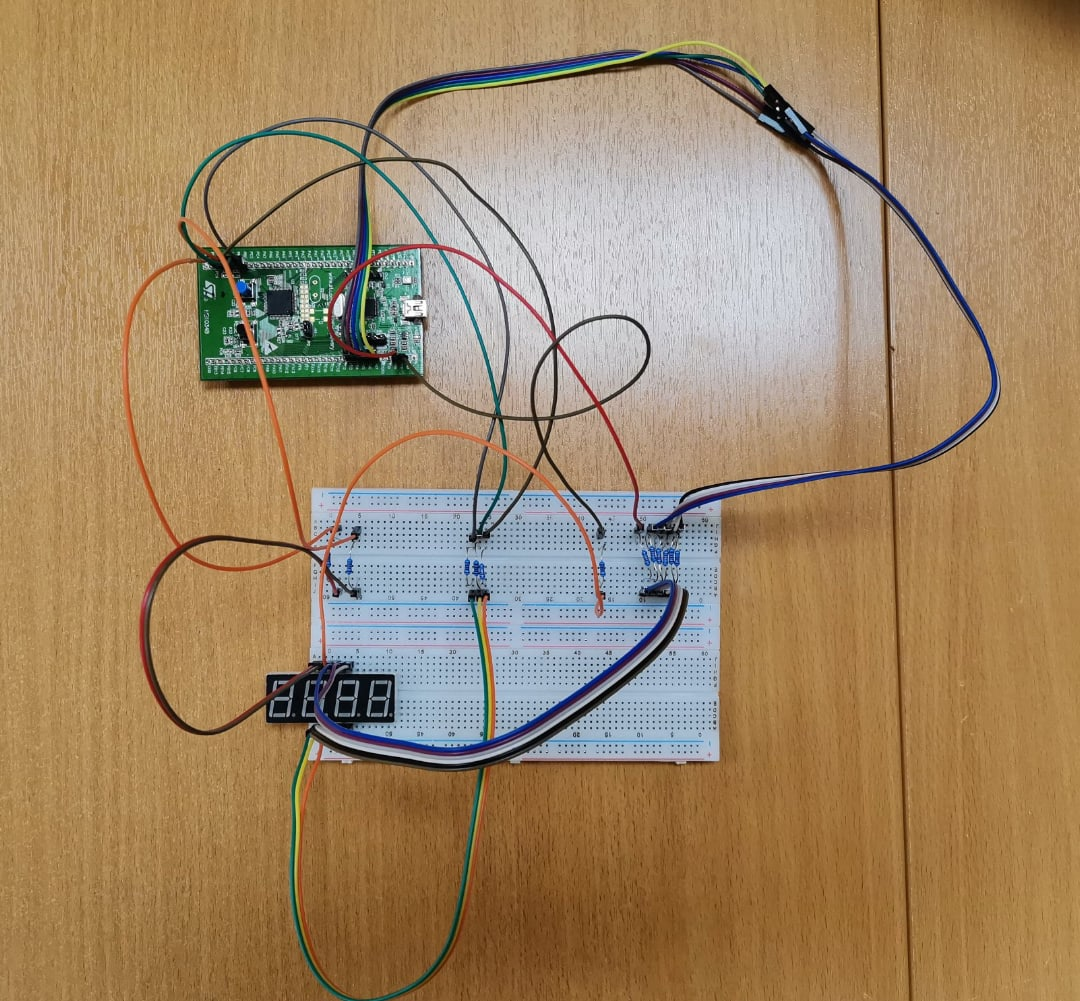
\includegraphics[width=0.8\linewidth]{pics/photo_of_stm.png}
		\caption{}
		\label{stm}
\end{figure}

\begin{figure}[h!]
		\centering
		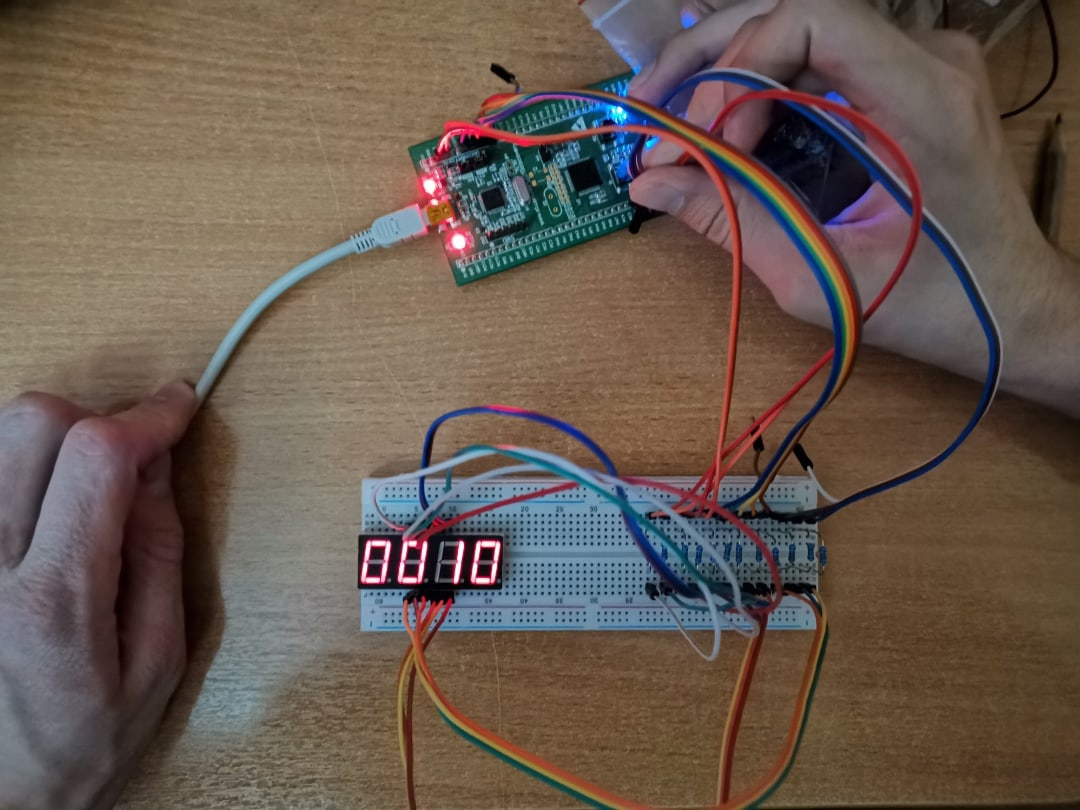
\includegraphics[width=0.8\linewidth]{pics/otl10.png}
		\caption{}
		\label{otl10}
\end{figure}

\newpage


\section{Кнопка:}


\import{./files/}{button.tex}

\newpage

\section{Семисегметный индикатор}

\import{./files/}{ind.tex}

\newpage

\section{Программная реализация нашего проекта на языке С с применением
         интегрированной среды разработки IAR for ARM}

\subsection{Бегущая строка}

\import{./files/}{show_str.tex}

\newpage

\subsection{Счетчик нажатий кнопки}

\import{./files/}{clicker.tex}


\end{document}